\section{Robustness against white noise}
\label{sec:noise}

The aim of this section is to study robustness against the addition of white
noise in a communication channel. The noise of the quantum channel is denoted by
$\alpha$, and thus we define the accuracy of the channel by $\mathcal{V} = 1 -
\alpha$, e.g. and accuracy of $\mathcal{V} = 1$ corresponds to a lossless
quantum channel. In experiments using a singlet state generated by two entangled
photons, the noise can originate from imperfect operations on the photon source
and detectors. Hence generating a pure singlet state is very difficult in
practice.\\

This noise effect can be modeled by the following mixed state, called a Werner state,
\begin{equation}\label{eq:werner-state}
    \rho = \mathcal{V} \ket{\Phi}\bra{\Phi} + (1-\mathcal{V}) \mathbbm{1}\text{ ,}
\end{equation}
where $\ket{\Phi}$ is a maximally entangled state and $\mathbbm{1}$ a fully
randomized behaviour.

The aim is to check for which amount of noise this state produces nonlocal behaviour
in CHSH and Mayers-Yao scenario.
The study of the robustness against white noise can be done by two different
manners :
\begin{enumerate}
    \item Start with  $\mathcal{V} = 1$ and a given precision $\delta$. While
        the result of the primal is an $\alpha > 0$, i.e., the behaviour $\mathcal P$ generated by $\rho$ and ideal measurements is non local, set
        $\mathcal{V} = \mathcal{V} - \delta $. This simple algorithm is useful
        to draw a curve as shown in \Autoref{fig:curve-noise}, but requires
        to solve $O(\delta^{-1})$ nonlinear problems, which is not time-wise negligible.

    \item Knowing that the visibility $\mathcal{V}$ is in the range $[0, 1]$, and
        that there exists a minimal value $\mathcal{V}^*$ such that for all
        $\mathcal{V} > \mathcal{V}^*$, the behaviour $\mathcal P$ generated with state $\rho$ (\Autoref{eq:werner-state}) and ideal measurements is not local, one can use a binary search
        to find $\mathcal{V}^*$ . This allows to proceed with a logarithmic
        number of iterations and an arbitrary large precision e.g., a twenty-digit
        accuracy with only 55 iterations. 
\end{enumerate}



The implementation of the first method yielded the curves represented in 
\Autoref{fig:curve-noise}.

\begin{Figure}
\centering
% This file was created with tikzplotlib v0.10.1.
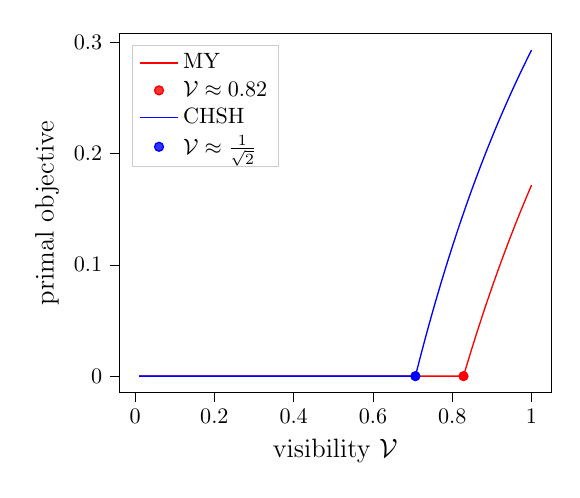
\begin{tikzpicture}[scale=.8]

\definecolor{darkgray176}{RGB}{176,176,176}
\definecolor{red}{RGB}{255,0,0}
\definecolor{lightgray204}{RGB}{204,204,204}

\begin{axis}[
legend cell align={left},
legend style={
  fill opacity=0.8,
  draw opacity=1,
  text opacity=1,
  at={(0.03,0.97)},
  anchor=north west,
  draw=lightgray204
},
tick align=outside,
tick pos=left,
x grid style={darkgray176},
xlabel={\large visibility \(\displaystyle \mathcal V\)},
xmin=-0.0395000000000008, xmax=1.0495,
xtick style={color=black},
y grid style={darkgray176},
ylabel={\large primal objective},
ymin=-0.0146446609406726, ymax=0.307537879754125,
ytick style={color=black}
]
\addplot [semithick, red]
table {%
1 0.17157287525381
0.99 0.163204924498798
0.98 0.154666199238581
0.97 0.145951417787433
0.96 0.137055078389385
0.95 0.127971447635589
0.94 0.118694548142351
0.93 0.109218145434204
0.92 0.0995357339715324
0.91 0.0896405222569338
0.9 0.0795254169486775
0.89 0.069183005903157
0.88 0.0586055400611474
0.87 0.0477849140848387
0.86 0.0367126456439648
0.85 0.0253798532397762
0.84 0.0137772324450116
0.83 0.00189503042627678
0.82 0
0.81 0
0.8 0
0.79 0
0.78 0
0.77 0
0.76 0
0.75 0
0.74 0
0.73 0
0.72 0
0.71 0
0.7 0
0.69 0
0.68 0
0.67 0
0.66 0
0.65 0
0.64 0
0.63 0
0.62 0
0.61 0
0.6 0
0.59 0
0.58 0
0.57 0
0.56 0
0.55 0
0.54 0
0.53 0
0.52 0
0.51 0
0.5 0
0.49 0
0.48 0
0.47 0
0.46 0
0.45 0
0.44 0
0.429999999999999 0
0.419999999999999 0
0.409999999999999 0
0.399999999999999 0
0.389999999999999 0
0.379999999999999 0
0.369999999999999 0
0.359999999999999 0
0.349999999999999 0
0.339999999999999 0
0.329999999999999 0
0.319999999999999 0
0.309999999999999 0
0.299999999999999 0
0.289999999999999 0
0.279999999999999 0
0.269999999999999 0
0.259999999999999 0
0.249999999999999 0
0.239999999999999 0
0.229999999999999 0
0.219999999999999 0
0.209999999999999 0
0.199999999999999 0
0.189999999999999 0
0.179999999999999 0
0.169999999999999 0
0.159999999999999 0
0.149999999999999 0
0.139999999999999 0
0.129999999999999 0
0.119999999999999 0
0.109999999999999 0
0.0999999999999992 0
0.0899999999999992 0
0.0799999999999993 0
0.0699999999999993 0
0.0599999999999993 0
0.0499999999999993 0
0.0399999999999993 0
0.0299999999999992 0
0.0199999999999992 0
0.00999999999999925 0
};
\addlegendentry{MY}
\addplot [semithick, red, mark=*, mark size=2, mark options={solid}, only marks]
table {%
0.828428781600444 0
};
\addlegendentry{$\mathcal V \approx 0.82$}
\addplot [semithick, blue]
table {%
1 0.292893218813452
0.99 0.285750726074194
0.98 0.278462468176992
0.97 0.271023936921085
0.96 0.263430436264013
0.95 0.255677072435213
0.94 0.247758743418566
0.93 0.2396701277564
0.92 0.231405672623318
0.91 0.222959581113684
0.9 0.214325798681614
0.89 0.2054979986668
0.88 0.196469566833469
0.87 0.187233584843049
0.86 0.177782812573782
0.85 0.168109669192297
0.84 0.158206212873158
0.83 0.148064119052352
0.82 0.137674657089576
0.81 0.127028665201793
0.8 0.116116523516815
0.79 0.104928125080319
0.78 0.093452844632631
0.77 0.0816795049525354
0.76 0.0695963405440161
0.75 0.0571909584179363
0.74 0.0444502956938543
0.73 0.0313605737170578
0.72 0.0179072483520168
0.71 0.00407495607528462
0.7 0
0.69 0
0.68 0
0.67 0
0.66 0
0.65 0
0.64 0
0.63 0
0.62 0
0.61 0
0.6 0
0.59 0
0.58 0
0.57 0
0.56 0
0.55 0
0.54 0
0.53 0
0.52 0
0.51 0
0.5 0
0.49 0
0.48 0
0.47 0
0.46 0
0.45 0
0.44 0
0.429999999999999 0
0.419999999999999 0
0.409999999999999 0
0.399999999999999 0
0.389999999999999 0
0.379999999999999 0
0.369999999999999 0
0.359999999999999 0
0.349999999999999 0
0.339999999999999 0
0.329999999999999 0
0.319999999999999 0
0.309999999999999 0
0.299999999999999 0
0.289999999999999 0
0.279999999999999 0
0.269999999999999 0
0.259999999999999 0
0.249999999999999 0
0.239999999999999 0
0.229999999999999 0
0.219999999999999 0
0.209999999999999 0
0.199999999999999 0
0.189999999999999 0
0.179999999999999 0
0.169999999999999 0
0.159999999999999 0
0.149999999999999 0
0.139999999999999 0
0.129999999999999 0
0.119999999999999 0
0.109999999999999 0
0.0999999999999992 0
0.0899999999999992 0
0.0799999999999993 0
0.0699999999999993 0
0.0599999999999993 0
0.0499999999999993 0
0.0399999999999993 0
0.0299999999999992 0
0.0199999999999992 0
0.00999999999999925 0
};
\addlegendentry{CHSH}
\addplot [semithick, blue, mark=*, mark size=2, mark options={solid}, only marks]
table {%
0.707108195400103 0
};
\addlegendentry{$\mathcal V \approx \frac{1}{\sqrt{2}}$}
\end{axis}

\end{tikzpicture}
\captionof{figure}{Optimal value of the linear program, depending on the set of correlations.}
\label{fig:curve-noise}
\end{Figure}

Concerning the CHSH's correlations, we obtained
\begin{equation*}
    \mathcal V ^*_{CHSH} \approx 0.71  \approx \frac{1}{\sqrt{2}}\text{ ,}
\end{equation*}
while comparatively, Mayer-Yao's correlations yield
\begin{equation*}
\mathcal{V}^*_{MY} \approx 0.82\text{ .}
\end{equation*}
As a conclusion, the maximally entangled state is more robust
to noise for CHSH correlations than for Mayers-Yao's correlations. The value $
\mathcal{V}^*$ can be interpreted as the visibility lower bound, meaning that if
the amount of noise is lower than $1-\mathcal{V}^*$, the violation of a Bell
inequality remains detectable in an experiment.

Besides, experiments reproducing the maximum violation of a Bell inequality for the CHSH
game have been realized without the need of calibrated devices
\cite{shadbolt2012}, and the experimental visibility they observed matches with
our result.

In each case, one can notice that $\mathcal{V}^* = 1 - \alpha^*$ where
$\alpha^*$ was the optimal objective obtained in \Autoref{sec:nonloc-detection}.
The study of the robustness is equivalent to the primal detecting non-local
behaviour since it was written using a convex combination of the behaviour and a
fully randomized behaviour, which is actually a white noise. Therefore, the
optimal value $\alpha^*$ of the primal corresponds to the maximal amount of noise 
tolerated for violating the Bell inequality. Still, this study would be necessary
whenever one wants to study different kinds of noise or losses arising from experimental setups: specific noises can be modeled as specific local behaviours, instead of only white noise \cite{shadbolt2012}.
% \hft{maybe arbitrary noise that is local, but normally just white noise.}